\documentclass[math,code]{amznotes}
\setcounter{tocdepth}{2}  % Only show sections in the ToC
\usepackage[utf8]{inputenc}
\usepackage{amsmath}
\usepackage{amsfonts}
\usepackage{graphicx}
\usepackage{tikz}
\usepackage{etoolbox}
\usepackage{tabularx}
\usepackage{float} % Needed for [H] placement specifier
\usepackage{wrapfig} % Needed for wrapping figures

\graphicspath{ {./images/} }
\geometry{
    a4paper,
    headheight = 1.5cm
}

\patchcmd{\chapter}{\thispagestyle{plain}}{\thispagestyle{fancy}}{}{}

\theoremstyle{remark}
\newtheorem*{claim}{Claim}
\newtheorem*{remark}{Remark}
\newtheorem{case}{Case}

\begin{document}
\fancyhead[L]{
    Engineering Calculus
}
\fancyhead[R]{
    Lecture Notes
}
\tableofcontents

\chapter{Partial Derivatives}
\section{Functions of Several Variables}
\subsection{Functions of Two variables}
\begin{dfnbox}{Functions of Two Variables}{function-of-two-variables}
    A function $\symbfit{f}$ of two variables is a rule that assigns to each ordered pair of real numbers $(x,y)$ in a set $\symbfit{D}$ a {\color{red} \textbf{unique}} real number denoted by $f(x,y)$. The set $D$ is the {\color{red} \textbf{domain}} of $f$ and its {\color{red} \textbf{range}} is the set of values that $f$ takes on, that is
    \begin{displaymath}
        \left\{ \, f(x,y) \mid (x,y) \in \symbfit{D} \, \right\}
    \end{displaymath}
\end{dfnbox}
We often write $z=f(x,y)$ to make explicit the value taken on by $\symbfit{f}$ at the general point $(x,y)$. The variables $\symbfit{x}$ and $\symbfit{y}$ are {\color{red} \textbf{independent variables}} and $\symbfit{z}$ is the {\color{red} \textbf{dependent variable}}.
\begin{notebox}
    \begin{remark}
        Compare this with the notation $y=f(x)$ for functions of a {\color{red} \textbf{single variable}}.
    \end{remark}
\end{notebox}
\subsection{Visualization}
Let's take functions of two variables as an example.
\begin{exbox}{Arrow Diagram for Functions of Two Variables}{arrow-diagram}
    A function of two variables is just a function whose domain is a subset of $\R^2$ and whose range is a subset of $R$. Then, we can draw the arrow diagram like below:
    \begin{figure}[H]
    \centering
    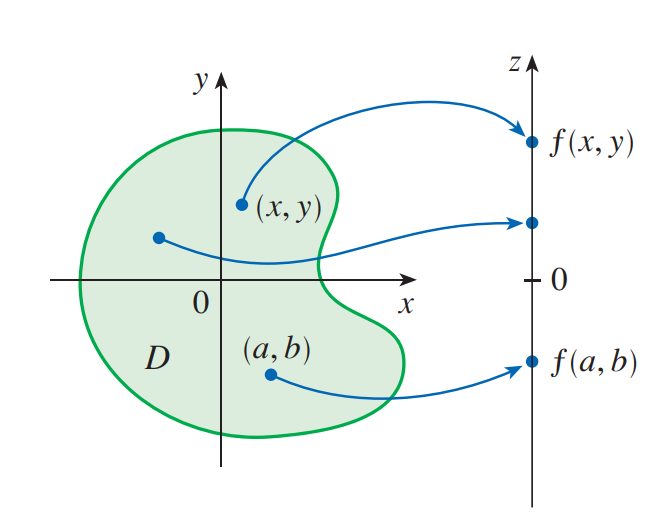
\includegraphics[width=0.35\linewidth]{images/arrow-diagram.png}
    \caption{Arrow Diagram}
    \label{fig:arrow-diagram}
    \end{figure}
\end{exbox}
\subsection{Graph}
Knowing the figure \ref{fig:arrow-diagram}, we can reform the diagram into a three dimensional coordinate system. And here comes the definition of \textbf{graph}
\begin{dfnbox}{Graph of functions of two variables}{graph-of-function-of-two-variables}
    If $\symbfit{f}$ is a function of two variables within domain $\symbfit{D}$, then the {\color{red} \textbf{graph}} of $\symbfit{f}$ is the set of all points $(x,y,z)$ in $\R^3$ such that $\symbfit{z}=f(x,y)$ and $(x,y)$ is in $\symbfit{D}$.
\end{dfnbox}
\begin{notebox}
    \begin{remark}
        Usually we can think $\symbfit{z}$ and $\symbfit{f(x,y)}$ are the same.
    \end{remark}
\end{notebox}
Now, let's see an example about how the graph for a function of two variables looks like.
\begin{exbox}{Graph of functions of two variables}{graph}
    In this figure \ref{fig:graph}, the area $\symbfit{S}$ is the graph of a function of two variables.
    \begin{figure}[H]
        \centering
        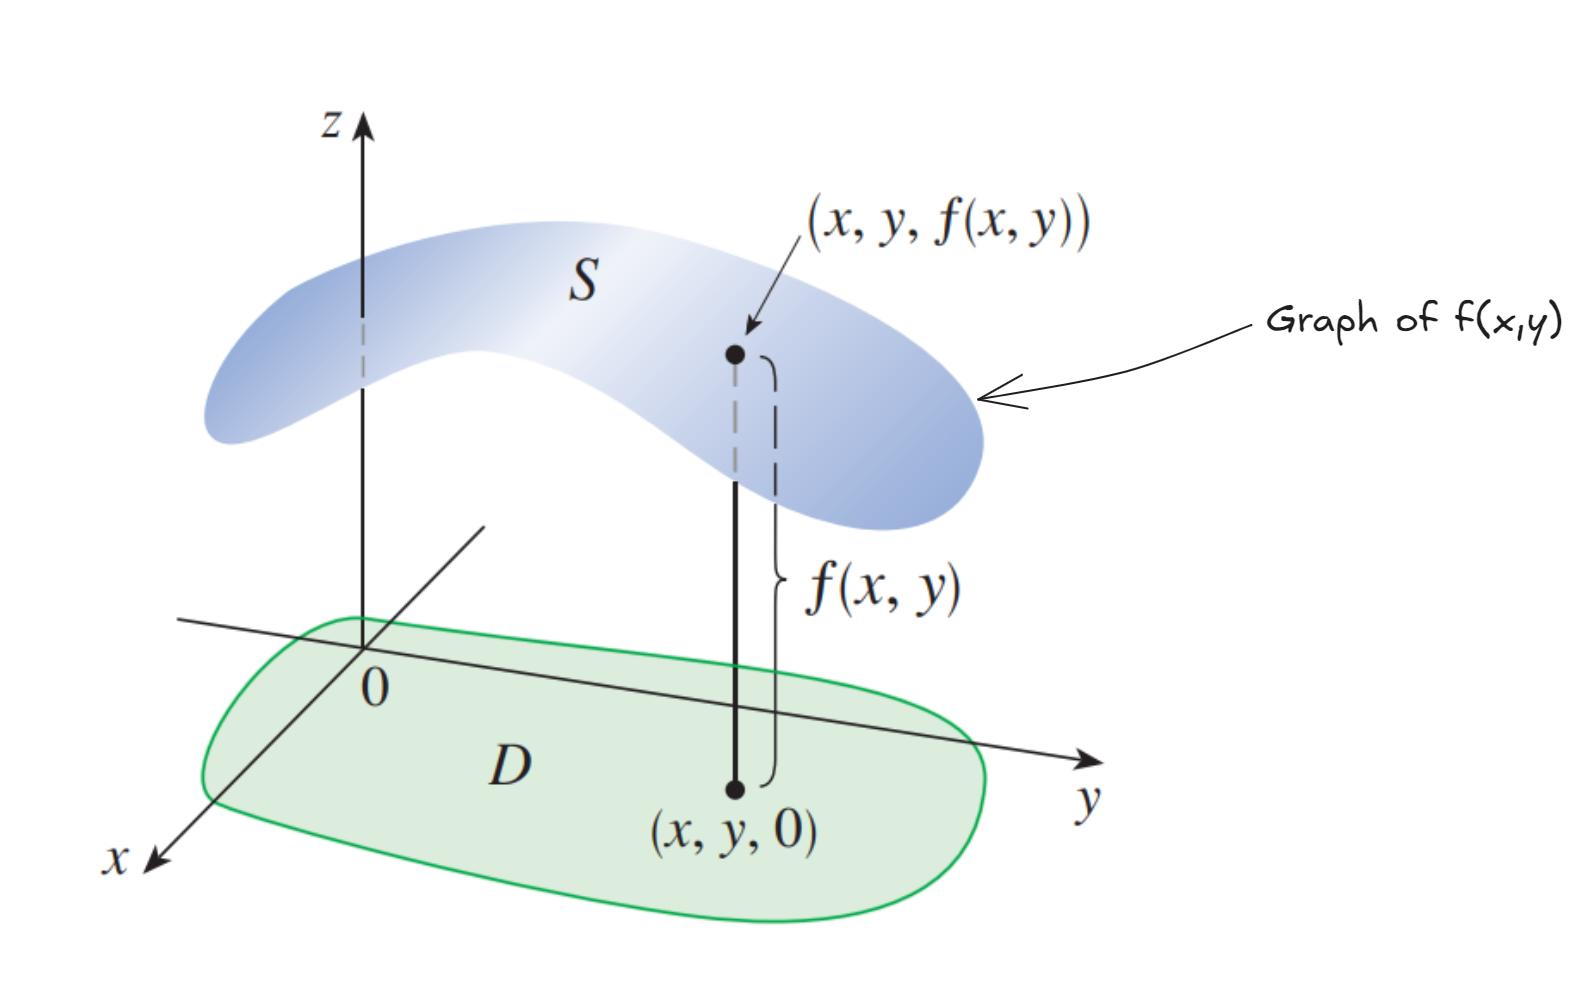
\includegraphics[width=0.5\linewidth]{images/graph.png}
        \caption{Graph}
        \label{fig:graph}
    \end{figure}
\end{exbox}
\begin{notebox}
    \begin{remark}
        In this example, the graph of the function is a \textbf{surface}. Graph is a more general concept and we can think that \textit{surface} is just one kind of \textit{graph} of a function.
    \end{remark}
\end{notebox}
\subsection{Level Curves}
\begin{dfnbox}{Level Curve}{levelcurve}
    The {\color{red} \textbf{level curves}} of a function $\symbfit{f}$ of two variables are the curves with equations $f(x,y)=\symbfit{k}$, where $\symbfit{k}$ is a constant (in the range of $\symbfit{f}$).
\end{dfnbox}
\begin{notebox}
    \begin{remark}
        From the definition of \nameref{dfn:levelcurve}, we should notice that a {\color{red} \textbf{level curve}} is the set of points in the domain of $\symbfit{f}$ at which $\symbfit{f}$ takes on a given value $\symbfit{k}$. In other words, it is a curve in {\color{red} $\symbfit{xy}$-plane} that shows where the graph of $\symbfit{f}$ has height $\symbfit{k}$ (above or below the $\symbfit{xy}$-plane).
    \end{remark}
\end{notebox}
\begin{exbox}{Find Level Curves}{findlevelcurves}
    Sketch the level curves of the function $f(x,y)=6-3x-2y$ for the values $k=-6,0,6,12$ \newline
    {\color{blue} \textbf{Solution}}: We just need to solve $6-3x-2y=k$, where $k=-6,0,6,12$. And then we will get four equations of line. We just need to plot these four lines out.
    \begin{figure}[H]
        \centering
        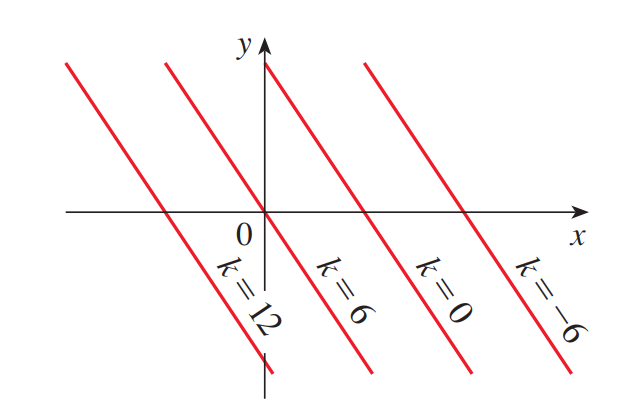
\includegraphics[width=0.5\linewidth]{images/level-curve-example.png}
        \caption{Level Curve Examples}
        \label{fig:level-curve-examples}
    \end{figure}
    In this example, we have a function of two variables and its graph should be in $\R^3$, but since we need to find its level curves. To find level curves, we need to decrease the dimension by 1, so its level curves are in $\R^2$.
\end{exbox}
\subsection{Contour Curves}
In the functions of two variables, we've seen that its level curves must be in $\R^2$. But thinking it deeply, how does level curves come? Basically, it is the projection of \textbf{contour curves} onto the $\symbfit{xy}$-plane. So, what is the \textbf{contour plane}?
\begin{dfnbox}{Contour Curve}{contourcurve}
    For a function of two variables, denoted by $z=f(x,y)$. A horizontal plane $z=k$ may or may not intersect with the graph of $\symbfit{f}$ along a curve. If the curve exists, we say that the curve is a {\color{red} \textbf{contour curve of height $k$}}. If not, we say the contour curve doesn't exist at height $k$ for the function $\symbfit{f}$.
\end{dfnbox}
To visual it more directly, let's see the example below
\begin{exbox}{Contour Curves Example}{contour-curve-examples}
    In this figure \ref{fig:contour-curves-example}, the \textit{horizontal races} are the same as \textit{contour curves} we've discussed above.
    \begin{figure}[H]
        \centering
        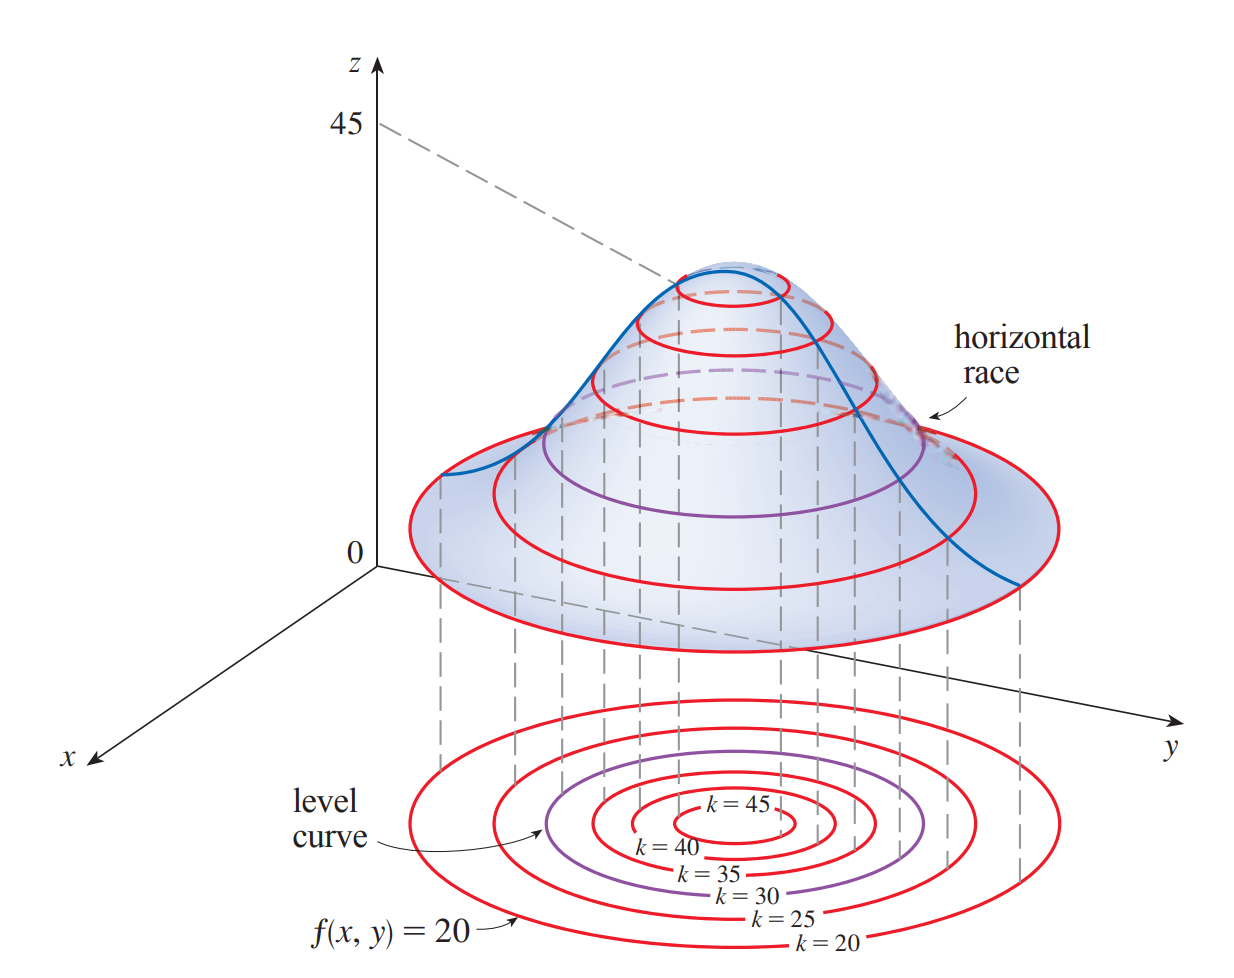
\includegraphics[width=0.5\linewidth]{images/contour-curve-example.png}
        \caption{Contour Curves Example}
        \label{fig:contour-curves-example}
    \end{figure}
\end{exbox}
\begin{notebox}
    \begin{remark}
        Sometimes, contour curves are also called \textbf{contour maps}.
    \end{remark}
\end{notebox}
\subsection{Functions of Three of more variables}
It's very difficult to visualize a function $f$ of three variables by its graph, since that would lie in $\R^4$. However, we do gain some insight into $f$ by examining its {\color{red} \textbf{level surfaces}}, which are surfaces with equations $f(x,y,z)=k$, where $k$ is a constant.
\begin{exbox}{Find level surfaces}{find-level-surfaces}
    Find the level surfaces of the function
    \begin{displaymath}
        f(x,y,z)=x^2+y^2+z^2
    \end{displaymath}
    {\color{blue} \textbf{Solution}}: The level surfaces are
    \begin{displaymath}
        x^2+y^2+z^2=k, ~where~ k\geq 0
    \end{displaymath}
    These form a family of concentric spheres of the function.
\end{exbox}

\section{Limits and Continuity}
\subsection{Limits}
\begin{dfnbox}{Limits}{limits}
    Let $\symbfit{f}$ be a function of two variables whose domain $\symbfit{D}$ includes points arbitrarily close to $(a,b)$. Then we say that the {\color{red} \textbf{limits of $f(x,y)$} as $(x,y)$ approaches $(a,b)$} is $\symbfit{L}$ and we write
    \begin{displaymath}
        \lim\limits_{(x,y) \to (a,b)} f(x,y) = L
    \end{displaymath}
    if for every number $\epsilon > 0$ there is a corresponding number $\delta > 0$ such that if $(x,y) \in D$ and $0 < \sqrt{(x-a)^2+(y-b)^2} < \delta$, then $\mid f(x,y) - L \mid < \epsilon$
\end{dfnbox}
\begin{exbox}{Explanation of Limits Definition}{explanation-limits-definition}
    Basically, it says that the distance between $f(x,y)$ and $L$ can be made arbitrarily small by making the distance from $(x,y)$ to $(a,b)$ sufficiently small, but not $0$. Let's form its arrow diagram as below,
    \begin{figure}[H]
        \centering
        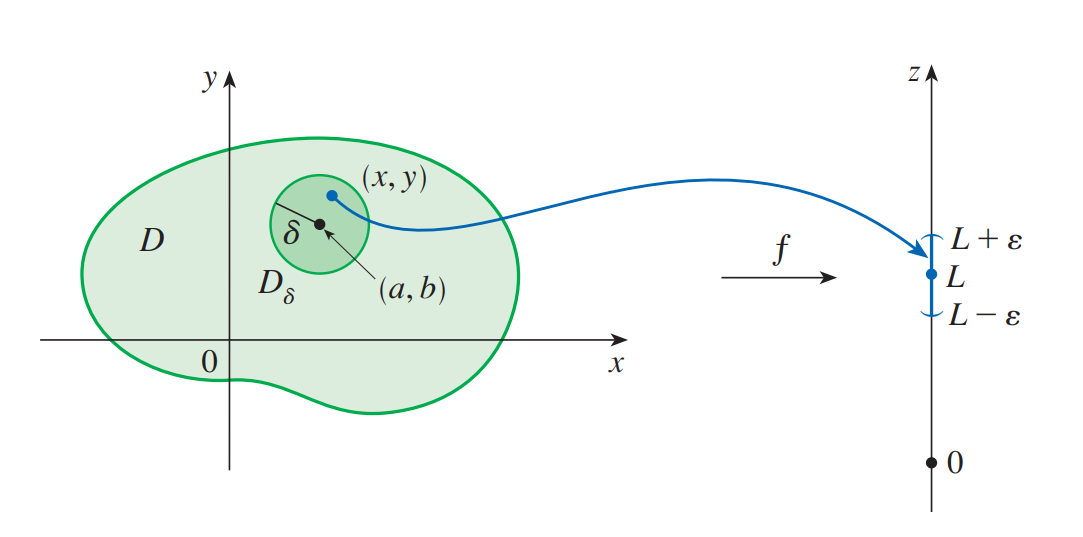
\includegraphics[width=0.5\linewidth]{images/limits-illustration.png}
        \caption{Limits Definition Explanation}
        \label{fig:limits-definition-explanation}
    \end{figure}
    From this figure \ref{fig:limits-definition-explanation}, we can see that if any small interval $(L - \epsilon, L + \epsilon)$ is given around $L$, then we can find a disk $D_\delta$ with center $(a,b)$ and radius $\delta > 0$ such that $\symbfit{f}$ maps all the points in $D_\delta$ \text{[except possibly $(a,b)$]} into the interval $(L - \epsilon, L + \epsilon)$
\end{exbox}
\subsubsection{Show that a limit doesn't exist}
Since in the definition of \nameref{dfn:limits}, it refers only to the \textbf{distance} between $(x,y)$ and $(a,b)$. It does not refer to the \textbf{direction} of approach. Therefore, if the limit exists, then $f(x,y)$ must approach the same limit \textbf{no matter how} $(x,y)$ approaches $(a,b)$. Thus, one way to show that $\lim_{(x,y) \to (a,b)} f(x,y)$ does not exist is to find {\color{red} \textbf{different paths}} of approach along which the function has different limits.
\begin{notebox}
    \begin{claim}
        If $f(x,y) \to L_1$ as $(x,y) \to (a,b)$ along a path $C_1$ and $f(x,y) \to L_2$ as $(x,y) \to (a,b)$ along a path $C_2$, where $L_1 \neq L_2$, then $\lim_{(x,y) \to (a,b)} f(x,y)$ does not exist.
    \end{claim}
\end{notebox}
\begin{exbox}{Limit does not exist}{limits-dne}
    Show that $\lim\limits_{(x,y) \to (0,0)} \frac{x^2-y^2}{x^2+y^2}$ does not exist \newline
    {\color{blue} \textbf{Solution}}:
    \begin{enumerate}
        \item Let's approach $(0,0)$ along the $x$-axis. On this path $y=0$, the function becomes $f(x,0)=\frac{x^2}{x^2}=1, \forall x \neq 0$ and thus
        \begin{displaymath}
            f(x,y) \to 1 \text{ as } (x,y) \to (0,0) \text{ along the }x \text{-axis.}
        \end{displaymath}
        \item We now approach along the $y$-axis by putting $x=0$. Then $f(0,y)=\frac{-y^2}{y^2}=-1, \forall y \neq 0$, so
        \begin{displaymath}
            f(x,y) \to -1 \text{ as } (x,y) \to (0,0) \text{ along the }y \text{-axis.}
        \end{displaymath}
        So, DNE!
    \end{enumerate}
\end{exbox}
\subsubsection{Properties of Limits}
Before we talk about the properties, let's give two definitions about the \textbf{polynomial function} and the \textbf{rational function}.
\begin{dfnbox}{Polynomial Function}{polynomial-function}
    A {\color{red} \textbf{polynomial function}} of two variables (or polynomial, for short) is a sum of terms of the form ($x^my^n$, where $\symbfit{c}$ is a constant and $\symbfit{m}$ and $\symbfit{n}$ are \textbf{non-negative integers}. For example,
    \begin{displaymath}
        p(x,y)=x^4+5x^3y^2+6xy^4-7y+6
    \end{displaymath}
\end{dfnbox}
\begin{dfnbox}{Rational Function}{rational-function}
    A {\color{red} \textbf{rational function}} is a ratio of two \nameref{dfn:polynomial-function}s. For example,
    \begin{displaymath}
        q(x,y)=\frac{2xy+1}{x^2+y^2}
    \end{displaymath}
\end{dfnbox}
Now, we state that
\begin{notebox}
    \begin{claim}
        To find the limit of any polynomial function, we can use \textbf{direct substitution}. For example,
        \begin{displaymath}
            \lim\limits_{(x,y) \to (a,b)} p(x,y) = p(a,,b)
        \end{displaymath}
    \end{claim}
\end{notebox}
and,
\begin{notebox}
    \begin{claim}
        To find the limit of any rational function, we have
        \begin{displaymath}
            \lim\limits_{(x,y) \to (a,b)} q(x,y) = \lim\limits_{(x,y) \to (a,b)} \frac{p(x,y)}{r(x,y)} = \frac{p(a,b)}{r(a,b)}=q(a,b)
        \end{displaymath}
        provided that $(a,b)$ is in the domain of $q$. If not, we need to use the definition about limits does not exist.
    \end{claim}
\end{notebox}
\subsection{Continuity}
\begin{dfnbox}{Continuity}{continuity}
    A function $\symbfit{f}$ of two variables is called {\color{red} \textbf{continuous}} at $(a,b)$ if
    \begin{displaymath}
        \lim\limits_{(x,y) \to (a,b)} f(x,y) = f(a,b)
    \end{displaymath}
    We say that $\symbfit{f}$ is {\color{red} \textbf{continuous}} on $\symbfit{D}$ if $\symbfit{f}$ is continuous at every point $(a,b)$ in $\symbfit{D}$.
\end{dfnbox}
\section{Partial Derivatives}
\subsection{First Order Partial Derivatives}
\subsubsection{Definition}
\begin{dfnbox}{First Order Partial Derivatives}{first-order-partial-derivative}
    If $\symbfit{f}$ is a function of two variables, its {\color{red} \textbf{partial derivative}} are the functions $f_x$ and $f_y$ defined by
    \begin{gather*}
        f_x(x,y)=\lim\limits_{h \to 0} \frac{f(x+h,y)-f(x,y)}{h} \\
        f_y(x,y)=\lim\limits_{h \to 0} \frac{f(x,y+h)-f(x,y)}{h}
    \end{gather*}
\end{dfnbox}
\subsubsection{Notation for Partial Derivatives}
If $z=f(x,y)$, we write
\begin{gather*}
    f_x(x,y)=f_x=\frac{\partial f}{\partial x}=\frac{\partial}{\partial x}f(x,y)=\frac{\partial z}{\partial x}=f_1=D_1f=D_xf \\
    f_y(x,y)=f_x=\frac{\partial f}{\partial y}=\frac{\partial}{\partial y}f(x,y)=\frac{\partial z}{\partial y}=f_2=D_2f=D_yf
\end{gather*}
\subsubsection{Rule for Finding Partial Derivatives of $z=f(x,y)$}
\begin{thmbox}{Rules for Finding First Order Partial Derivatives}{find-first-order-partial}
    \begin{enumerate}
        \item To find $f_x$, regard $\symbfit{y}$ as a constant and differentiate $f(x,y)$ with regard to $\symbfit{x}$.
        \item To find $f_y$, regard $\symbfit{x}$ as a constant and differentiate $f(x,y)$ with regard to $\symbfit{y}$.
    \end{enumerate}
\end{thmbox}
\subsubsection{Rules of Differentiation}
Since when doing partial differentiation, we are treating one variable as a constant (if we have two variables in total), so the rules of differentiation for single variable still applies. Let's recap them.
\begin{thmbox}{Rules of Differentiation}{rules-of-differentiation}
    \begin{gather*}
        (fg)' = f'g+g'f \text{ (product rule)} \\
        (\frac{f}{g})'=\frac{f'g-g'f}{g^2} \text{ (quotient rule)} \\
        (f \circ g)' = f'(g) \cdot g' \text{ (chain rule) } ~~\text{where}~~ (f \circ g)(x) = f(g(x)) 
    \end{gather*}
\end{thmbox}
\subsubsection{Geometric Meaning of First Order Partial Derivatives} \label{sec:geometric-meaing-of-first-order-partial-deri}
$f_x(a,b)$ and $f_y(a,b)$ can be interpreted geometrically as the {\color{red} \textbf{slopes}} of the tangent lines at $P(a,b,c)$ to the traces $C_1$ and $C_2$ of $\symbfit{S}$ in the plane $y=b$ and $x=a$
\begin{figure}[H]
    \centering
    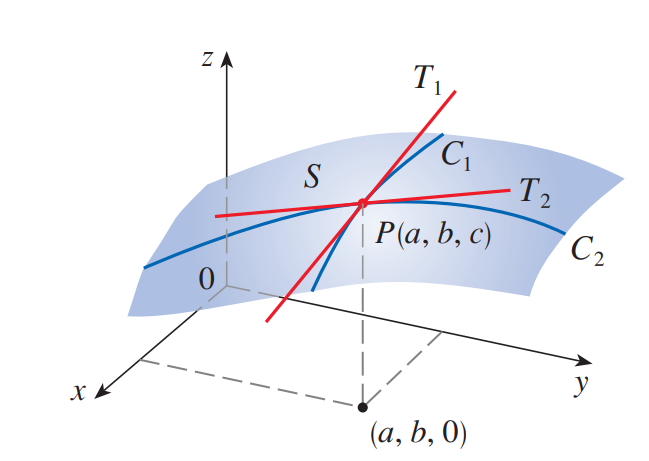
\includegraphics[width=0.3\linewidth]{images/partial-derivative-geometric-meaning.png}
    \caption{Geometric Meaning of First order Partial Derivatives}
    \label{fig:geo-meaning-first-order-partial-derivative}
\end{figure}
\begin{notebox}
    \begin{remark}
        Note that \textbf{slopes} are numbers, so the first order partial derivative should be a \textit{number} as well, but this \textit{number} can be in real number form or in the expression form.
    \end{remark}
\end{notebox}
\begin{exbox}{Implicit Partial Differentiation}{implicit-partial-diff}
    Find $\partial z / \partial x$ and $\partial z / \partial y$ if $\symbfit{z}$ is defined implicitly as a function of $\symbfit{x}$ and $\symbfit{y}$ by the equation
    \begin{displaymath}
        x^3+y^3+z^3+6xyz+4=0
    \end{displaymath}
    {\color{blue} \textbf{Solution}}:
    \begin{enumerate}
        \item We differentiate implicitly with regard to $\symbfit{x}$, being careful to treat $\symbfit{y}$ as a constant and $\symbfit{z}$ as a function (of $\symbfit{x}$)
        \begin{displaymath}
            3x^2+3z^2\frac{\partial z}{\partial x}+\underbrace{6yz+6xy\frac{\partial z}{\partial x}}_\text{Product Rule! Be careful!}=0
        \end{displaymath}
        Solving this equation, we get
        \begin{displaymath}
            \frac{\partial z}{\partial x}=-\frac{x^2+2yz}{z^2+2xy}
        \end{displaymath}
        \item Similarly, we implicitly differentiate with regard to $\symbfit{y}$, we will get
        \begin{displaymath}
            \frac{\partial z}{\partial y}=-\frac{y^2+2xz}{z^2+2xy}
        \end{displaymath}
    \end{enumerate}
\end{exbox}
\subsection{Higher Order Partial Derivatives}
If $\symbfit{f}$ is a function of two variables, then its partial derivatives $f_x$ and $f_y$ are also functions of two variables, so we can consider their partial derivatives $(f_x)_x, (f_x)_y, (f_y)_x, (f_y)_y$, which are called {\color{red} \textbf{second partial derivatives}} of $\symbfit{f}$. If $z=f(x,y)$, we use the following notation:
\begin{gather*}
    (f_x)_x=f_{xx}=f_{11}=\frac{\partial}{\partial x}(\frac{\partial f}{\partial x})=\frac{\partial ^2 f}{\partial x^2}=\frac{\partial ^2 z}{\partial x^2} \\
    (f_x)_y=f_{xy}=f_{12}=\frac{\partial}{\partial y}(\frac{\partial f}{\partial x})=\frac{\partial ^2 f}{\partial y \partial x}=\frac{\partial ^2 z}{\partial y \partial x} \\
    (f_y)_x=f_{yx}=f_{21}=\frac{\partial}{\partial x}(\frac{\partial f}{\partial y})=\frac{\partial ^2 f}{\partial x \partial y}=\frac{\partial ^2 z}{\partial x \partial y} \\
    (f_y)_y=f_{yy}=f_{22}=\frac{\partial}{\partial y}(\frac{\partial f}{\partial y})=\frac{\partial ^2 f}{\partial y^2}=\frac{\partial ^2 z}{\partial y^2}
\end{gather*}
A very useful Theorem,
\begin{thmbox}{Clairaut's Theorem}{clairaut-theorem}
    Suppose $\symbfit{f}$ is defined on a disk $\symbfit{D}$ that contains the point $(a,b)$. If the functions $f_{xy}$ and $f_{yx}$ are both continuous on $\symbfit{D}$, then:
    \begin{displaymath}
        f_{xy}(a,b)=f_{yx}(a,b)
    \end{displaymath}
    This theorem is sometimes called {\color{red} \textbf{The Mixed Derivative Theorem}}.
\end{thmbox}
\section{Tangent Planes and Linear Approximations}
\subsection{Tangent Planes}
\subsubsection{What is a tangent plane}
\begin{dfnbox}{Tangent Plane}{tangent-plane}
    Let $P(x_0,y_0,z_0)$ be a point on the surface $\symbfit{S}$ defined by the equation $z=f(x,y)$. We will see that the {\color{red} \textbf{tangent plane}} to $\symbfit{S}$ at $\symbfit{P}$ consists of {\color{red} \textbf{all}} tangent lines at $\symbfit{P}$ to curves that lie on $\symbfit{S}$ and pass through $\symbfit{P}$.
\end{dfnbox}
For example, let $\symbfit{C_1}$ and $\symbfit{C_2}$ be the curves obtained by intersecting the vertical planes $y=y_0$ and $x=x_0$ with the surface $\symbfit{S}$. Let $\symbfit{T_1}$ and $\symbfit{T_2}$ be the tangent lines to the curves $\symbfit{C_1}$ and $\symbfit{C_2}$ at point $\symbfit{P}$. Then the {\color{red} \textbf{tangent plane}} to the surface $\symbfit{S}$ at the point $\symbfit{P}$ is defined to be the plane that contains both tangent lines $\symbfit{T_1}$ and $\symbfit{T_2}$. (See figure \ref{fig:tangent-plane})
\begin{figure}[H]
    \centering
    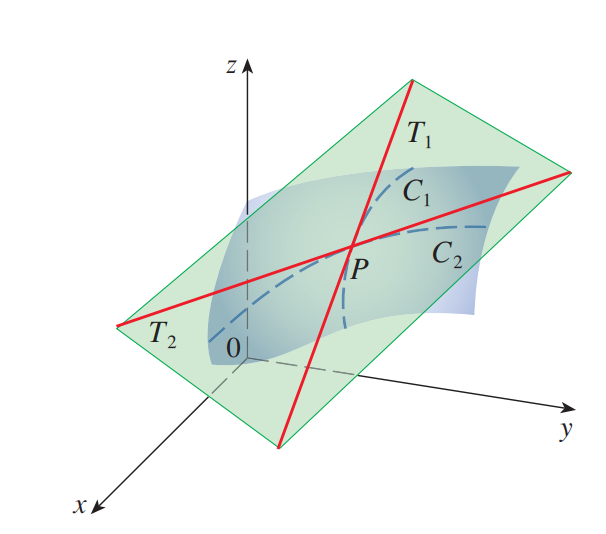
\includegraphics[width=0.3\linewidth]{images/tangent-plane.png}
    \caption{Tangent Plane}
    \label{fig:tangent-plane}
\end{figure}
\subsubsection{Derive the equation of a tangent plane}
\begin{enumerate}
    \item We know that any plane passing through the point $P(x_0,y_0,z_0)$ has an equation of the form:
    \begin{displaymath}
        A(x-x_0)+B(y-y_0)+C(z-z_0)=0
    \end{displaymath}
    \item By dividing this equation by $\symbfit{C}$ and letting $a=-A/C, b=-B/C$, we can write it in the form:
    \begin{equation} \label{eq:plane-intermediate}
        z-z_0=a(x-x_0)+b(y-y_0)
    \end{equation}
    \item If equation \eqref{eq:plane-intermediate} represents the tangent plane at $\symbfit{P}$, then its intersection with the plane $y=y_0$ must be the tangent line $\symbfit{T_1}$. Setting $y=y_0$ in Equation \eqref{eq:plane-intermediate} gives
    \begin{displaymath}
        z-z_0=a(x-x_0) ~~~\text{where}~ y=y_0
    \end{displaymath}
    \item We recognize this as the equation (in point-slope form) of a line with slope $\symbfit{a}$. But from beforehand (see this section about \ref{sec:geometric-meaing-of-first-order-partial-deri} the geometric meaning of first order partial derivatives), we know that the slope of the tangent line $T_1$ is $f_x(a,b)$. Therefore,
    \begin{displaymath}
        a=f_x(a,b)
    \end{displaymath}
    \item Similarly, we can get
    \begin{displaymath}
        b=f_y(a,b)
    \end{displaymath}
\end{enumerate}
Now, let's see the {\color{red} \textbf{Equation of a Tangent Plane}}
\begin{thmbox}{Equation of a Tangent plane}{tangent-plane-equation}
    Suppose $\symbfit{f}$ has continuous partial derivatives. An equation of the tangent plane to the surface $z=f(x,y)$ at the point $P(x_0,y_0,z_0)$ is
    \begin{equation} \label{eq:equation-of-tangent-plane-special}
        z-z_0=f_x(x_0,y_0)(x-x_0)+f_y(x_0,y_0)(y-y_0)
    \end{equation}
\end{thmbox}
\begin{notebox}
    \begin{remark}
        Note that the similarity between the equation of a tangent plane and the equation of a tangent line:
        \begin{displaymath}
            y-y_0=f'(x_0)(x-x_0)
        \end{displaymath}
        This will help you memorize the \nameref{thm:tangent-plane-equation}
    \end{remark}
\end{notebox}
\subsection{Linear Approximations}
\begin{dfnbox}{Linearization}{Linearization}
    The linear function whose graph is this tangent plane, namely
    \begin{displaymath}
        L(x,y)=f(a,b)+f_x(a,b)(x-a)+f_y(a,b)(y-b)
    \end{displaymath}
    is called a {\color{red} \textbf{linearization}} of $\symbfit{f}$ at $(a,b)$ and the approximation,
    \begin{displaymath}
        f(x,y) \approx f(a,b)+f_x(a,b)(x-a)+f_y(a,b)(y-b)
    \end{displaymath}
    is called {\color{red} \textbf{linear approximation}} or the {\color{red} \textbf{tangent plane approximation}} of $\symbfit{f}$ at $(a,b)$.
\end{dfnbox}
\begin{notebox}
    \begin{remark}
        Note that the linear function $L(x,y)$ and the original function $\symbfit{f}$ are {\color{red} \textbf{not}} the same function!
    \end{remark}
\end{notebox}
\subsection{Differentiable function of two variables}
\begin{dfnbox}{Differentiable function of two variables}{differentiable-function-of-two-variables}
    If $z=f(x,y)$, then $\symbfit{f}$ is {\color{red} \textbf{differentiable}} at $(a,b)$ if $\Delta z$ can be expressed in the form
    \begin{displaymath}
        \Delta z = f_x(a,b)\Delta x+f_y(a,b)\Delta y + \epsilon_1\Delta_x + \epsilon_2\Delta_y
    \end{displaymath}
    where $\epsilon_1$ and $\epsilon_2$ are functions of $\Delta_x$ and $\Delta_y$ such that $\epsilon_1$ and $\epsilon_2 \to 0$ as $(\Delta_x,\Delta_y) \to 0$
\end{dfnbox}
Sometimes it is hard to use the Definition of \nameref{dfn:differentiable-function-of-two-variables} to directly check the {\color{red} \textbf{differentiability}} of a function, but below provides a convenient {\color{red} \textbf{sufficient}} condition for differentiability.
\begin{thmbox}{Differentiability Test}{differentiability-test}
    If the partial derivatives $f_x$ and $f_y$ exist near $(a,b)$ and are continuous at (a,b), then $f$ is differentiable at $(a,b)$
\end{thmbox}
\subsection{Differentials}
\begin{dfnbox}{Differential}{differential}
    For a differential function of two variables, $z=f(x,y)$, we define the {\color{red} \textbf{differentials}} $dx$ and $dy$ to be independent variables; that is, they can be given any values. Then the {\color{red} \textbf{differential}} $dz$, also called the {\color{red} \textbf{total differential}}, is defined by
    \begin{equation} \label{eq:two-varaibles-differentials}
        dz=f_x(x,y)dx+f_y(x,y)dy=\frac{\partial z}{\partial x}\cdot dx+\frac{\partial z}{\partial y}\cdot dy
    \end{equation}
\end{dfnbox}
\subsubsection{Geometric meaning of $dz$ and $\Delta z$}
Figure \ref{fig:geomertic-meaning-of-differential-two-variables} shows the geometric interpretation of the differential $dz$ and the increment $\Delta z$: $dz$  represents the change in height of the tangent plane, whereas $\Delta z$ represents the change in height of the surface $z=f(x,y)$ when $(x,y)$ changes from $(a,b)$ to $(a+\Delta x, b+\Delta y)$
\begin{figure}[H]
    \centering
    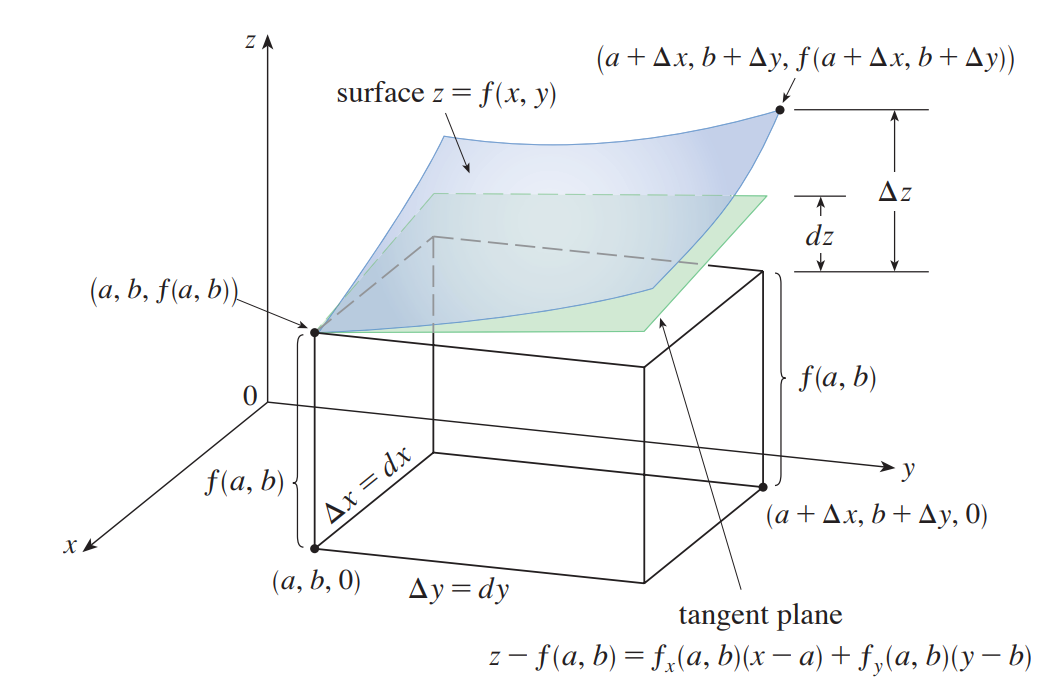
\includegraphics[width=0.5\linewidth]{images/geomertic-meaning-of-differential-two-variables.png}
    \caption{Geometric Meaning of Differentials (Two variables)}
    \label{fig:geomertic-meaning-of-differential-two-variables}
\end{figure}
\begin{exbox}{Use differentials to approximate}{differential-approximation}
    \begin{enumerate}
        \item If $z=f(x,y)=x^3+3xy-y^2$, find the differential $dz$
        \item If $x$ changes from $2$ to $2.05$ and $y$ changes from $3$ to $2.96$, compare the values of $\Delta z$ and $dz$
    \end{enumerate}
    {\color{blue} Solution}:
    \begin{enumerate}
        \item Definition of $dz$ gives that
        \begin{align*}
            dz&=\frac{\partial z}{\partial x}\cdot dx+\frac{\partial z}{\partial y}\cdot dy \\
            &=(2x+3y)\cdot dx+(3x-2y)\cdot dy  
        \end{align*}
        \item Putting $x=2, dx=\Delta x=0.05, y=3$ and $dy=\Delta y=-0.04$, we get
        \begin{align*}
            dz&=[2(2)+3(3)]\cdot 0.05+[3(2)-2(3)]\cdot (-0.04) \\
            &=0.65
        \end{align*}
        The increment of $z$ is:
        \begin{align*}
            \Delta z &= f(2.05,2.96)-f(2,3) \\
            &\approx0.6449
        \end{align*}
    \end{enumerate}
    Notice that $\Delta z \approx dz$ but $dz$ is easier to compute.
\end{exbox}
\subsubsection{How to memorize}
For a differential function of one variable, $y=f(x)$, we define the differential $dx$ to be an independent variable; that is $dx$ can be given the value of any real number. The differential of $y$ is then defined as:
\begin{equation} \label{eq:one-variable-differential}
    dy = f'(x)dx
\end{equation}
And its geometric interpretation can be shown in figure \ref{fig:geometric-meaning-of-differential-one-variable}
\begin{figure}[H]
    \centering
    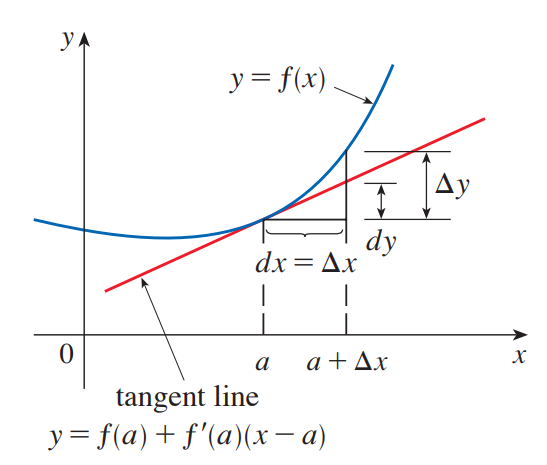
\includegraphics[width=0.4\linewidth]{images/geometric-meaning-of-differential-one-variable.png}
    \caption{Geometric Meaning of Differential (One variable)}
    \label{fig:geometric-meaning-of-differential-one-variable}
\end{figure}
We can compare Equation \eqref{eq:one-variable-differential} with \eqref{eq:two-varaibles-differentials}, so that we can memorize the two variables one easily.
\section{Chain Rule and Implicit Differentiation}
\subsection{Chain Rule with one Independent Variable}
One Independent Variable means that, for example $z$ indirectly a function of $t$.
\begin{thmbox}{Chain Rule (Case 1)}{chain-rule-case-1}
    Suppose that $z=f(x,y)$ is a differentiable function of $x$ and $y$, where $x=g(t)$ and $y=h(t)$ are both differentiable functions of $t$. Then $z$ is a differentiable function of $t$ and
    \begin{align} 
        \frac{dz}{dt}&=\frac{\partial f}{\partial x}\cdot \frac{dx}{dt}+\frac{\partial f}{\partial y}\cdot \frac{dy}{dt} \label{eq:chain-rule-case-1} \\ 
        \xRightarrow{\partial f \to \partial z} &= \frac{\partial z}{\partial x}\cdot\frac{dx}{dt} +\frac{\partial z}{\partial y}\cdot \frac{dy}{dt}
    \end{align}
\end{thmbox}
\begin{notebox}
    \begin{remark}
        Notice the similarity between \eqref{eq:chain-rule-case-1} and the definition of differentials of functions of two variables in \eqref{eq:two-varaibles-differentials}.
    \end{remark}
\end{notebox}
\subsection{Chain Rule with two Independent Variable}
Two Independent Variables means that, for example $z$ is indirectly a function of two variables, $s$ and $t$.
\begin{thmbox}{Chain Rule (Case 2)}{chain-rule-case-2}
    Suppose that $z=f(x,y)$ is a differentiable function of $x$ and $y$, where $x=g(s,t)$ and $y=h(s,t)$ are differentiable functions of $s$ and $t$, then
    \begin{gather*}
        \frac{\partial z}{\partial s}=\frac{\partial z}{\partial x} \cdot \frac{\partial x}{\partial s} + \frac{\partial z}{\partial y} \cdot \frac{\partial y}{\partial s} \\
        \frac{\partial z}{\partial t}=\frac{\partial z}{\partial t} \cdot \frac{\partial x}{\partial t} + \frac{\partial z}{\partial y} \cdot \frac{\partial y}{\partial t}
    \end{gather*}
\end{thmbox}
The following tree diagram may help you memorize this theorem.
\begin{figure}[H]
    \centering
    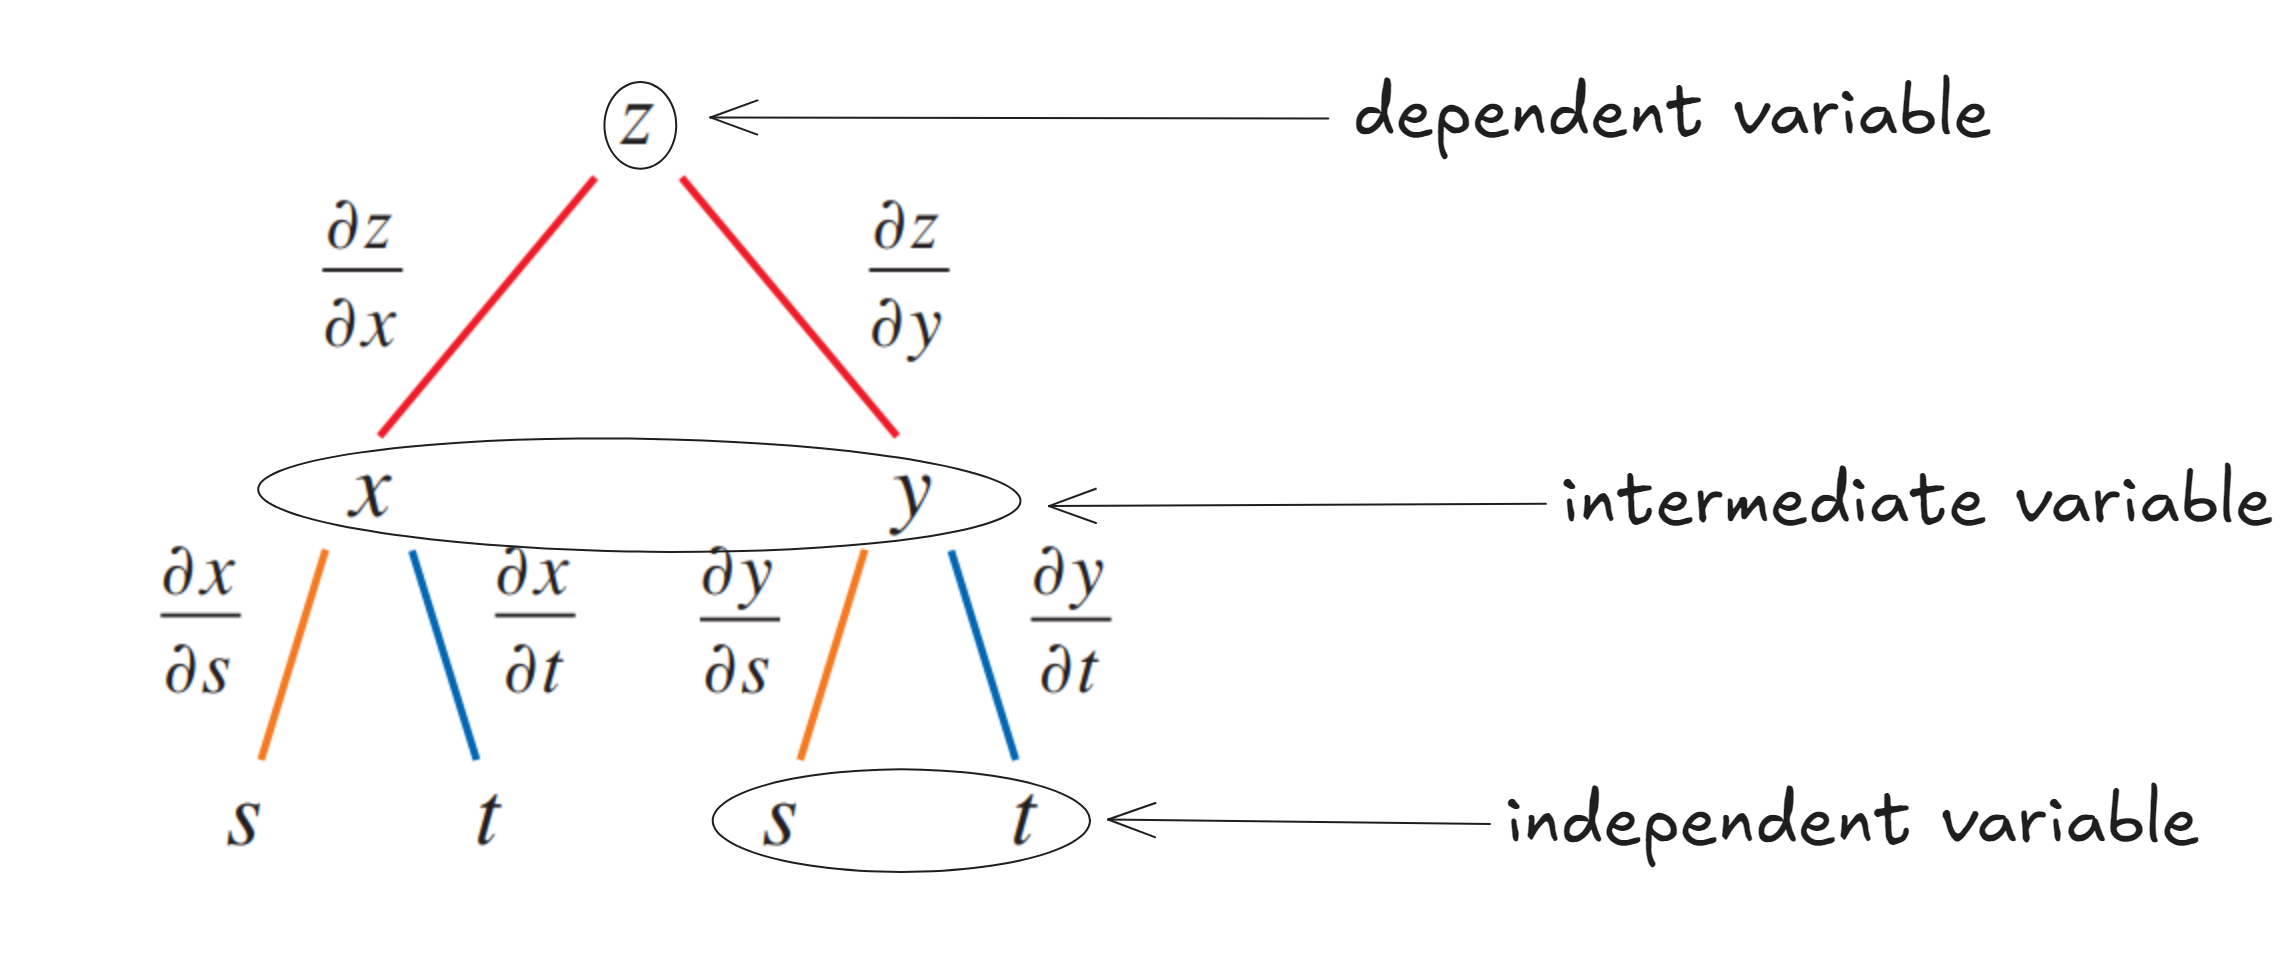
\includegraphics[width=0.5\linewidth]{images/chain-rule.png}
    \caption{Chain rule}
    \label{fig:chain-rule}
\end{figure}
\subsection{Implicit Differentiation}
\subsubsection{Single Independent Variable}
$y=f(x)$ where $F(x,f(x))=0$, for all $x$ in the domain of $\symbfit{f}$. Using \nameref{thm:chain-rule-case-1} to differentiate both sides of $F(x,y)=0$, we will get
\begin{displaymath}
    \frac{\partial F}{\partial x} \cdot \frac{dx}{dx} + \frac{\partial F}{\partial y} \cdot \frac{dy}{dx} = 0
\end{displaymath}
But $dx/dx = 1$, so if $\partial F / \partial y \neq 0$, we can obtain
\begin{equation} \label{eq:single-variable-implicit-function-theorem}
    \frac{dy}{dx} = - \frac{\frac{\partial F}{\partial x}}{\frac{\partial F}{\partial y}} = -\frac{F_x}{F_y}
\end{equation}
The equation \eqref{eq:single-variable-implicit-function-theorem} is called {\color{red} \textbf{Implicit Function Theorem}}
\begin{exbox}{Implicit Function Theorem Example}{implicit-function-theorem-example}
    Find $y'$ if $x^3+y^3=6xy$ \newline
    {\color{blue} \textbf{Solution}}:
    \begin{gather*}
        F(x,y)=x^3+y^3-6xy \\
        y'=\frac{dy}{dx}=-\frac{F_x}{F_y}=-\frac{3x^2-6y}{3y^2-6x}=-\frac{x^2-2y}{y^2-2x}
    \end{gather*}
\end{exbox}
\subsubsection{Two Independent Variables}
Use \nameref{thm:chain-rule-case-2} to differentiate both sides of $F(x,y,z)=0$
\begin{displaymath}
    \frac{\partial F}{\partial x} \cdot \frac{\partial x}{\partial x} + \frac{\partial F}{\partial y} \cdot \frac{\partial y}{\partial x} + \frac{\partial F}{\partial z} \cdot \frac{\partial z}{\partial x} = 0
\end{displaymath}
But $\partial x / \partial x = 1$ and $\partial y / \partial x = 0$, so this equation becomes
\begin{displaymath}
    \frac{\partial F}{\partial x} + \frac{\partial F}{\partial z} \cdot \frac{\partial z}{\partial x} = 0
\end{displaymath}
If $\partial F / \partial z \neq 0$, then we have
\begin{equation} \label{eq:two-variables-implicit-function-theorem-1}
    \frac{\partial z}{\partial x} = -\frac{\frac{\partial F}{\partial x}}{\frac{\partial F}{\partial z}} = - \frac{F_x}{F_z}
\end{equation}
Similarly, we can get
\begin{equation} \label{eq:two-variables-implicit-function-theorem-2}
    \frac{\partial z}{\partial y} = -\frac{\frac{\partial F}{\partial y}}{\frac{\partial F}{\partial z}} = - \frac{F_y}{F_z}
\end{equation}
Equation \eqref{eq:two-variables-implicit-function-theorem-1} and equation \eqref{eq:two-variables-implicit-function-theorem-2} form the other part of {\color{red} \textbf{Implicit Function Theorem}}.
\section{Directional Derivatives and the Gradient Vector}
\subsection{Directional Derivatives}
$f_x(x,y)$ and $f_y(x,y)$ give us the rate of change in the $x-$ and $y-$directions. But a {\color{red} \textbf{directional derivative}} enables us to find the rate of change of a function of two or more variables in {\color{red} \textbf{any direction}}.
\subsubsection{Definition of Directional Derivatives}
\begin{dfnbox}{Directional Derivative}{directional-derivative}
    The {\color{red} \textbf{directional derivative}} of $\symbfit{f}$ at $(x_0,y_0)$ in the direction of a unit vector $\langle a,b \rangle$ is
    \begin{equation}
        D_uf(x_0,y_0)=\lim\limits_{h \to 0} \frac{f(x_0+ha, y_0+hb)-f(x_0,y_0)}{h}
    \end{equation}
    If $u=i=\langle 1,0 \rangle$, then $D_if=f_x$, if $u=j=\langle 0,1 \rangle$, then $D_jf=f_y$. In other words, the partial derivatives of $\symbfit{f}$ with regard to $x$ and $y$ are just special cases of the directional derivatives.
\end{dfnbox}
\subsubsection{Geometric meaning of Directional Derivatives}
Suppose that we wish to o find the rate of change of $z$ at $x_0,y_0$ in the direction of an arbitrary unit vector $\symbfit{u}=\langle a,b \rangle$. To do this, we consider the surface $S$ with the equation $z=f(x,y)$ (the graph of $f$) and we let $z_0=f(x_0,y_0)$. Then, the point $P(x_0,y_0,z_0)$ lies on $S$. The vertical plane that passes through $P$ in the direction of $\symbfit{u}$ intersects $S$ in a curve $C$. (See Figure \ref{fig:geometric-meaing-of-directional-derivative}) The {\color{red} \textbf{slope}} of the tangent line $T$ to $C$ at the point $P$ is the rate of change of $z$ in the direction of $\symbfit{u}$.
\begin{figure}[H]
    \centering
    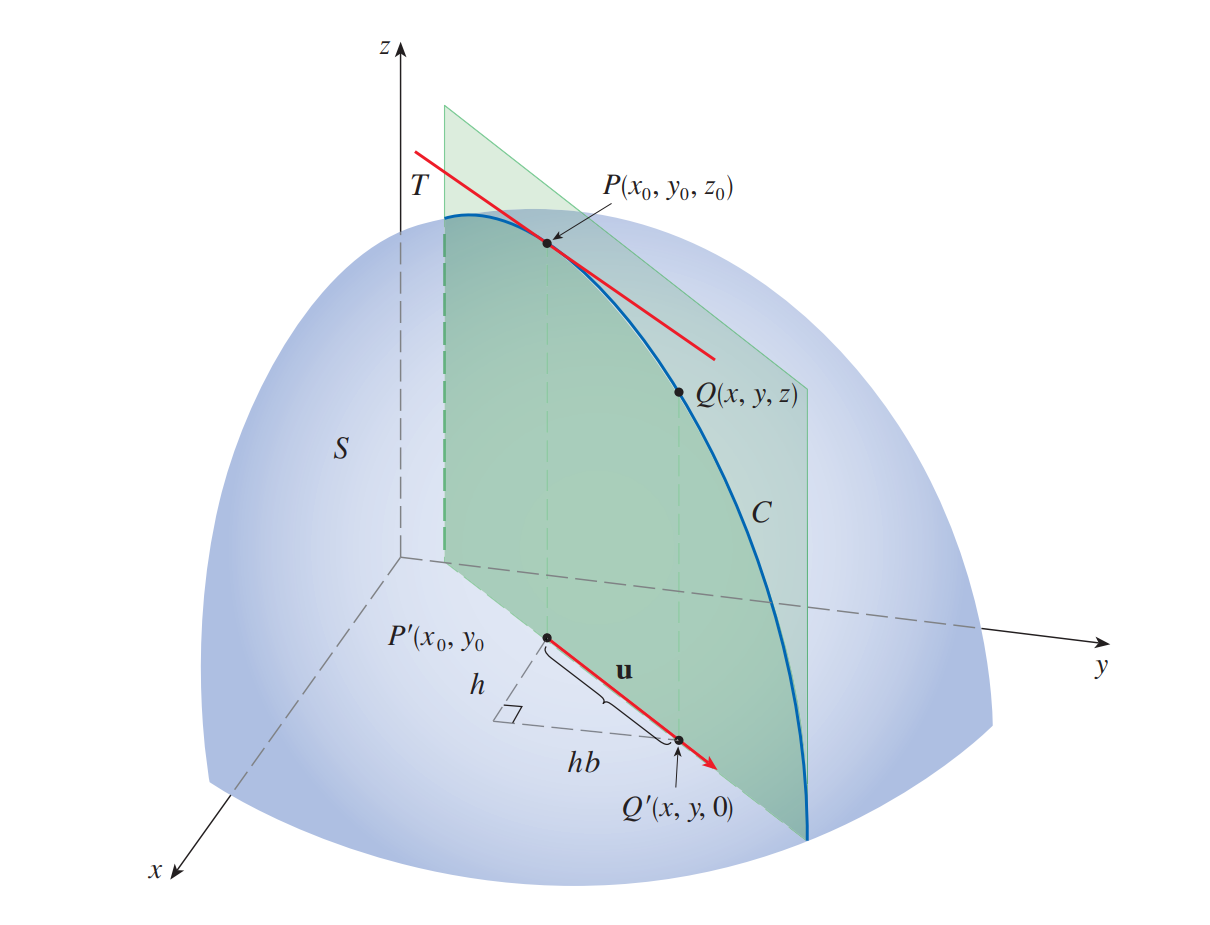
\includegraphics[width=0.5\linewidth]{images/geometric-meaing-of-directional-derivative.png}
    \caption{Geometric Meaning of Directional Derivatives}
    \label{fig:geometric-meaing-of-directional-derivative}
\end{figure}
\subsubsection{How to find the Directional Derivative}
\begin{thmbox}{Find Directional Derivatives}{find-directional-derivatives}
    If $\symbfit{f}$ is a differentiable function of $x$ and $y$, then $\symbfit{f}$ has a directional derivative in the direction of any unit vector $u=\langle a,b \rangle$ and
    \begin{displaymath}
        D_uf(x,y)=f_x(x,y)a+f_y(a,b)b
    \end{displaymath}
\end{thmbox}
\textbf{Proof of theorem \ref{thm:find-directional-derivatives}}: \newline
\begin{enumerate}
    \item Define a function $g(h)=f(x_0+ha, y_0+hb)$
    \item By the definition of a derivative, we have
    \begin{align}
        g'(0)&=\lim\limits_{h \to 0}\frac{g(h)-g(0)}{h} \\
        &=\lim\limits_{h \to 0}\frac{f(x_0+ha, y_0+hb)-f(x_0,y_0)}{h} \\
        &=D_uf(x_0,y_0) \label{eq:proof-direction-derivative-2}
    \end{align}
    \item On the other hand, we can write $g(h)=f(x,y)$ where $x=x_0+ha, y=y_0+hb$, so \nameref{thm:chain-rule-case-1} gives
    \begin{align*}
        g'(h)&=\frac{\partial f}{\partial x} \cdot \frac{dx}{dh} + \frac{\partial f}{\partial y]} \cdot \frac{dy}{dh} \\
        &=f_x(x,y)a+f_y(x,y)b
    \end{align*}
    \item Put $h=0, x=x_0, y=y_0$, we get
    \begin{equation} \label{eq:proof-directional-derivative-4}
        g'(0)=f_x(x_0,y_0)a + f_y(x_0,y_0)b
    \end{equation}
    \item Compare equation \eqref{eq:proof-direction-derivative-2} and equation \eqref{eq:proof-directional-derivative-4}, we prove that
    \begin{equation} \label{eq:directional-derivative-equation}
        D_uf(x_0,y_0)=f_x(x_0,y_0)a+f_y(x_0,y_0)b
    \end{equation}
\end{enumerate}
\subsection{Gradient Vector}
\subsubsection{Definition of Gradient Vector}
\begin{dfnbox}{Gradient Vector}{gradient-vector}
    If $f$ is a function of two variables $x$ and $y$, then the {\color{red} \textbf{gradient}} of $f$ is the vector function $\nabla f$ (grad $f$, or read "del $f$") defined by,
    \begin{displaymath}
        \nabla f(x,y)=\langle f_x(x,y), f_y(x,y) \rangle = \frac{\partial f}{\partial x}i+\frac{\partial f}{\partial y}j
    \end{displaymath}
\end{dfnbox}
\begin{notebox}
    \begin{remark}
        Note that with the $\nabla f$, we can rewrite the directional derivative equation \eqref{eq:directional-derivative-equation} as,
        \begin{equation}
            D_uf(x,y)=\nabla f(x,y) \cdot \symbfit{u}
        \end{equation}
        Where $\symbfit{u}$ is a unit vector.
    \end{remark}
\end{notebox}
\subsubsection{Maximizing the Directional Derivative}
Suppose $f$ is a differentiable function of two or three variables. The maximum value of the directional derivative $D_uf(x)$ is $|\nabla f(x)|$ and it occurs when $\symbfit{u}$ has the same direction as the gradient vector $\nabla f(x)$.
\begin{notebox}
    \begin{remark}
        Note that here $\symbfit{x}$ is a vector, and we use vector notation here.
    \end{remark}
\end{notebox}
{\textbf{Proof}}: \newline
Here we write the directional derivative at the point $(x_0, y_0)$ as the dot product, which will be
\begin{equation} \label{eq:proof-maximizing-directional-derivative}
    D_uf(x_0,y_0)=|\nabla f(x_0,y_0)| \cdot |u| \cdot cos(\theta)
\end{equation}
Where $\theta$ is the angle between vector $\nabla f$ and the unit vector $\symbfit{u}$. And since in the equation \eqref{eq:proof-maximizing-directional-derivative}, the only variable is $\theta$. We can quickly know that, max $cos(\theta)$ is 1. That means $\nabla f(x_0,y_0)$ has the same direction as the unit vector $\symbfit{u}$. Proof!
\subsubsection{Geometric Meaning of Gradient Vector}
Suppose $S$ is a surface with equation $F(x,y,z)=lk$, that is, it is a {\color{red} \textbf{level surface}} of function $F$ of {\color{red} \textbf{three}} variables, and let $P(x_0,y_0,z_0)$ be a point on $S$. Let $C$ be {\color{red} \textbf{any}} curve that lies on the surface $S$ and passes through the point $P$. We can describe the curve $C$ as a continuous vector function $r(t)=\langle x(t), y(t), z(t) \rangle$. Let $t_0$ be the parameter  value corresponding to $P$; that is $r(t_0)=\langle x_0, y_0, z_0 \rangle$. Since $C$ lies on $S$, any point $\langle x(t), y(t), z(t) \rangle$ must satisfy the equation of $S$, that is
\begin{displaymath}
    F(x(t), y(t), z(t))=k
\end{displaymath}
Use \nameref{thm:chain-rule-case-1} to differentiate both sides
\begin{displaymath}
    \frac{\partial F}{\partial x} \cdot \frac{dx}{dt} + \frac{\partial F}{\partial y} \cdot \frac{dy}{dt} + \frac{\partial F}{\partial z} \cdot \frac{dz}{dt} = 0
\end{displaymath}
But since, $\nabla F = \langle F_x, F_y, F_z \rangle$ and $r'(t) = \langle x'(t), y'(t), z'(t) \rangle$, so the above equation can be written as
\begin{displaymath}
    \nabla F \cdot r'(t) = 0
\end{displaymath}
In particular, when $t=t_0$, we have
\begin{equation} \label{eq:geometric-meaning-of-gradient-vector}
    \nabla F(x_0,y_0,z_0) \cdot r'(t_0) = 0
\end{equation}
This equation \eqref{eq:geometric-meaning-of-gradient-vector} says that the gradient vector at $P$, which is $\nabla F(x_0,y_0,z_0)$ is perpendicular to the {\color{red} \textbf{tangent vector}} $r'(t_0)$ to {\color{red} \textbf{any}} curve $C$ on $S$ that passes through $P$. If $\nabla F(x_0,y_0,z_0) \neq 0$, it is therefore natural to define the {\color{red} \textbf{tangent plane}} to the level surface $F(x,y,z) = k$ at $P(x_0,y_0,z_0)$ as the plane that
\begin{enumerate}
    \item passes through $P$
    \item and has the normal vector $\nabla F(x_0,y_0,z_0)$
\end{enumerate}
Thus, the equation of the tangent plane can be written as:
\begin{equation} \label{eq:equation-of-tangent-planes-general}
    F_x(x_0,y_0,z_0)(x-x_0) + F_y(x_0,y_0,z_0)(y-y_0) +F_z(x_0,y_0,z_0)(z-z_0) = 0
\end{equation}
\begin{figure}[H]
    \centering
    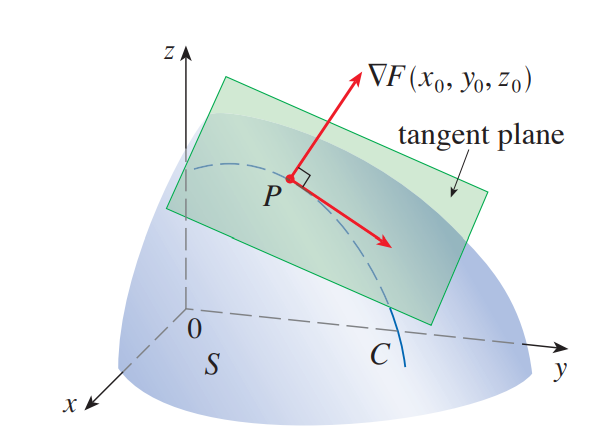
\includegraphics[width=0.5\linewidth]{images/geometric-meaing-of-gradient-vector.png}
    \caption{Geometric Meaning of Gradient Vector}
    \label{fig:geometric-meaing-of-gradient-vector}
\end{figure}
Now, we can define the {\color{red} \textbf{normal line}} to $S$ at $P$ to be the line passing through $P$ and perpendicular to the tangent plane. The direction of the normal line is therefore given by the gradient vector $\nabla F(x_0,y_0,z_0)$ and so, its symmetric equations are
\begin{displaymath}
    \frac{x-x_0}{F_x(x_0,y_0,z_0)} = \frac{y-y_0}{F_y(x_0,y_0,z_0)} = \frac{z-z_0}{F_z(x_0,y_0,z_0)}
\end{displaymath}
\subsubsection{Significance of Gradient Vectors}
Let $f$ be a differentiable function of two or three variables and suppose that $\nabla f(x) \neq 0$ (Here $\symbfit{x}$ is a vector)
\begin{enumerate}
    \item The directional derivative of $f$ at $x$ in the direction of a unit vector $\symbfit{u}$ is given by $D_uf(x)=\nabla f(x) \cdot \symbfit{u}$
    \item $\nabla f(x)$ points in the direction of maximum rate of increase of $f$ at $x$, and the maximum rate of change of $f$ is $|\nabla f(x)|$
    \item $\nabla f(x)$ is perpendicular to the {\color{red} \textbf{level curve or level surface}} of $f$ through $x$ \label{}
\end{enumerate}
\begin{notebox}
    \begin{remark}
    Notice the following important points:
        \begin{enumerate}
            \item Point 3 is also known as the {\color{red} \textbf{Geometric Meaning of Gradient Vectors}} (according to equation \eqref{eq:geometric-meaning-of-gradient-vector}).
            \item Using the point 3 to understand stand point 2 makes it more intuitive.
            \item In point 3, note that it is not the graph, but the level surface or level curve. But sometimes we can think the graph as level $\cdots$ by increasing $\R^n$ to $\R^{n+1}$
        \end{enumerate}
    \end{remark}
\end{notebox}
\subsubsection{Extend Tangent Planes}
Since we have derived a general equation \eqref{eq:equation-of-tangent-planes-general} for tangent plane. We may wonder whether the equation \eqref{eq:equation-of-tangent-plane-special} we have derived before still applies or not. Let's try to verify that. \newline
In the special case in which the equation of a surface $S$ is of the form $z=f(x,y)$ (that is $f$ is the graph of a function $f$ of two variables), we can rewrite the equation as
\begin{displaymath}
    F(x,y,z)=f(x,y)-z=0
\end{displaymath}
and regard $S$ as a {\color{red} \textbf{level surface}} (with $k=0$) of $F$. Then
\begin{gather*}
    F_x(x_0,y_0,z_0)=f_x(x_0,y_0) \\
    F_y(x_0,y_0,z_0)=f_y(x_0,y_0) \\
    F_z(x_0,y_0,z_0)=-1 
\end{gather*}
Substitute these into equation \eqref{eq:equation-of-tangent-planes-general}, we get,
\begin{displaymath}
    f_x(x_o,y_0)(x-x_0)+f_y(x_0,y_0)(y-y_0)-(z-z_0)=0
\end{displaymath}
which is equivalent to the equation \eqref{eq:equation-of-tangent-plane-special} we have derived before. Thus, our new, more general definition(equation) \eqref{eq:equation-of-tangent-planes-general} of a tangent plane is consistent with the definition(equation) that was given for the special case before.
\subsubsection{Normal Vectors under the special case tangent planes}
With the knowledge of gradient vectors, we can easily get the normal vector of the special case tangent plane (where the original function $f$ is a function of two variables) as below,
\begin{displaymath}
    \left[\begin{array}{c}
        f_x(a,b) \\
        f_y(a,b) \\
        -1
    \end{array}\right]
\end{displaymath}
is normal to the tangent plane at $P(a,b,f(a,b))$. And this vector is called the {\color{red} \textbf{Normal Vector}} of the tangent plane at $P(a,b,f(a,b))$. With this knowledge, we can get the vector equations of our tangent plane and normal line
\begin{thmbox}{Tangent Plane (Vector Equation)}{tangent-plane-vector-equations}
    A vector equation of the tangent plane at $\symbfit{P}$ is
    \begin{displaymath}
        \symbfit{r} \cdot \left[\begin{array}{c}
             f_x(a,b) \\
             f_y(a,b) \\
             -1
        \end{array}\right]
        =
        \left[\begin{array}{c}
             a \\
             b \\
             f(a,b)
        \end{array}\right]
        \cdot
        \left[\begin{array}{c}
             f_x(a,b) \\
             f_y(a,b) \\
             -1
        \end{array}\right]
    \end{displaymath}
\end{thmbox}
\begin{thmbox}{Normal Lines (Vector Equation)}{normal lines}
    The equation of the normal line at $\symbfit{P}$ (which is the line passing through $\symbfit{P}$ and perpendicular to the tangent plane) is
    \begin{displaymath}
        \symbfit{r} =
        \left[\begin{array}{c}
             a \\
             b \\
             f(a,b)
        \end{array}\right]
        +
        \left[\begin{array}{c}
             f_x(a,b) \\
             f_y(a,b) \\
             -1
        \end{array}\right]
        t, ~~~t \in \symbfit{R}
    \end{displaymath}
\end{thmbox}
\section{Maximum and Minimum Values}
\subsection{Local Maximum and Local Minimum Values}
\begin{thmbox}{Local Maximum or local minimum test}{local-maximum-minimum-test}
    If $f$ has a local maximum or minimum at $(a,b)$ and the first-order partial derivatives of $f$ exist there, then
    \begin{displaymath}
        f_x(a,b)=0 ~~~\text{and}~~~ f_y(a,b)=0
    \end{displaymath}
\end{thmbox}
\begin{notebox}
    \begin{remark}
        Note that using the gradient vector, the \nameref{thm:local-maximum-minimum-test} can be written as
        \begin{displaymath}
            \nabla f(a,b)=0
        \end{displaymath}
    \end{remark}
\end{notebox}
\subsubsection{Critical Point}
Extending our definition of critical point in single variable function, now let's extend our definition of critical points.
\begin{dfnbox}{Critical Point}{critical-point}
    A point $(a,b)$ is called a {\color{red} \textbf{critical point}} (or stationary point) of $f$ if
    \begin{enumerate}
        \item $f_x(a,b)=0$ and $f_y(a,b)=0$
        \item {\color{red} \textbf{or}} if one of these partial derivatives does not exist
    \end{enumerate}
\end{dfnbox}
\subsubsection{Saddle Point}
\begin{dfnbox}{Saddle Point}{saddle-point}
    If point $(a,b)$ is a \nameref{dfn:critical-point}, but $f(a,b)$ is neither a local maximum nor a local minimum, then point $(a,b)$ is called a {\color{red} \textbf{saddle point}}.
\end{dfnbox}
\subsubsection{Second Derivative Test}
Similar to the first derivative test that we use in single variable differentiation to indicate the local maximum/minimum information about a function. We also have a similar test called {\color{red} \textbf{Second Derivative Test}} to indicate the local maximum/minimum information about a function with two independent variables.
\begin{thmbox}{Second Derivative Test}{second-derivative-test}
    Suppose the second partial derivatives of $f$ are continuous on a disk with center $(a,b)$, and suppose that $f_x(a,b)=0$ and $f_y(a,b)=0$ [so $(a,b)$ is a critical point of $f$]. Let
    \begin{displaymath}
        D=D(a,b)=f_{xx}(a,b)f_{yy}(a,b)-[f_{xy}(a,b)]^2
    \end{displaymath}
    \begin{enumerate}
        \item If $D>0$ and $f_{xx}(a,b)>0$, then $f(a,b)$ is a {\color{red} \textbf{local minimum}}.
        \item If $D>0$ and $f_{xx}(a,b)<0$, then $f(a,b)$ is a {\color{red} \textbf{local maximum}}.
        \item If $D<0$, then $(a,b)$ is a {\color{red} \textbf{saddle point}} of $f$.
    \end{enumerate}
\end{thmbox}
\begin{notebox}
    \begin{remark}
        Note:
        \begin{enumerate}
            \item If $D=0$, the test gives no information: $f$ could have a local maximum or local minimum at $(a,b)$ or $(a,b)$ could be a saddle point of $f$.
            \item To remember the formula for $D$, it's helpful to write it as a determinant:
            \begin{displaymath}
                D =
                \begin{vmatrix}
                    f_{xx} & f_{xy} \\
                    f_{xy} & f_{yy}
                \end{vmatrix}
                = f_{xx}f_{yy} - (f_{xy})^2
            \end{displaymath}
        \end{enumerate}
    \end{remark}
\end{notebox}
\subsection{Absolute Maximum and Minimum Values}
Before we talk about it, let's look at two important concepts, {\color{red} \textbf{Closed Set}} and {\color{red} \textbf{Boundary Points}}
\subsubsection{Closed set}
\begin{dfnbox}{Closed Set}{closed-set}
    A {\color{red} \textbf{closed set}} in $\R^2$ is one that contains {\color{red} \textbf{all}} its \nameref{dfn:boundary-points}.
\end{dfnbox}
\subsubsection{Boundary Points}
\begin{dfnbox}{Boundary Points}{boundary-points}
    A {\color{red} \textbf{boundary point}} of $D$ is a point $(a,b)$ such that {\color{red} \textbf{every disk}} with center $(a,b)$ contains points in $D$ and also points not in $D$.
\end{dfnbox}
\begin{exbox}{Find boundary points}{find-boundary-points}
    $D=\{(x,y)\mid x^2+y^2 \leq 1\}$. Find its boundary points. \newline
    {\color{blue} \textbf{Solution}}: The points on the circle $x^2+y^2=1$ are all its boundary points.
\end{exbox}
This figure \ref{} shows the some examples of \nameref{dfn:closed-set}.
\begin{figure}[H]
    \centering
    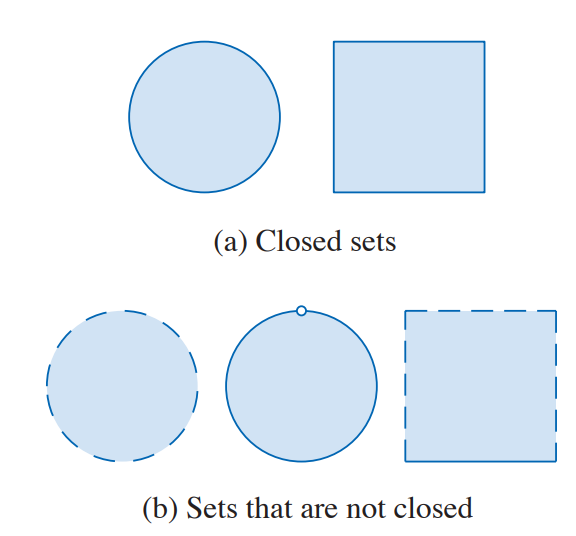
\includegraphics[width=0.5\linewidth]{images/closed-set-examples.png}
    \caption{Closed Sets and Not Closed Sets}
    \label{fig:closed-sets-example}
\end{figure}
\subsubsection{Extreme Value Theorem for Functions of Two variables}
Now, we can extend the extreme value theorem to functions of two variables.
\begin{thmbox}{Extreme Value Theorem (Functions of Two variables)}{evt-for-functions-of-two}
    If $f$ is continuous on a {\color{red} \textbf{closed, bounded set}} $D$ in $\R^2$, then $f$ attains an absolute maximum value $f(x_1,y_1)$ and an absolute minimum value $f(x_2,y_2)$ at some points $(x_1,y_1)$ and $(x_2,y_2)$ in $D$.  
\end{thmbox}
\subsubsection{Strategy to find absolute maximum/minimum values of a continuous functions $f$ on a closed, bounded set $D$}
\begin{enumerate}
    \item Find the values of $f$ at the {\color{red} \textbf{critical points}} of $f$ in $D$
    \item Find the extreme values of $f$ on the {\color{red} \textbf{boundary}} of $D$
    \item The largest of the values from steps 1 and 2 is the absolute maximum value; the smallest of these values is the absolute minimum values.
\end{enumerate}
\section{Lagrange Multipliers}
Sometimes we want to find the maximum/minimum value of a function under some constraint. This kind of problem is called \textbf{constrained optimized problem}. We may use the idea of \textit{eliminating variables} to solve this kind of question, but it is kind of tedious. And the following is an alternative approach to solving constrained optimization problems.
\subsection{One Constraint}
\subsubsection{Geometric Basis}
Let's start by trying to find the extreme values of $f(x,y)$ subject to a constraint of the form $g(x,y)=k$. In other words, we seek the extreme values of $f(x,y)$ when the point $(x,y)$ is restricted to lie on the level curve $g(x,y)=k$. Figure \ref{fig:geometric-meaning-lagrange-multiplier} shows this curve together with several level curves of $f$. These have the equations $f(x,y)=c$ where $c=7,8,9,10,11$. To maximize $f(x,y)$ subject to $g(x,y)=k$ is to find the largest value of $c$ such that the level curve $f(x,y)=c$ intersects $g(x,y)=k$. It appears from Figure \ref{fig:geometric-meaning-lagrange-multiplier} that this happens when these curves just touch each other, that is, when they have a common tangent line. (Otherwise, the value of $c$ could be increased further.) This means that the normal lines at the point $(x_0,y_0)$ where they touch are identical. So the gradient vectors are parallel; that is
\begin{displaymath}
    \nabla f(x_0,y_0)=\lambda \nabla g(x_0,y_0)
\end{displaymath}
\begin{figure}[H]
    \centering
    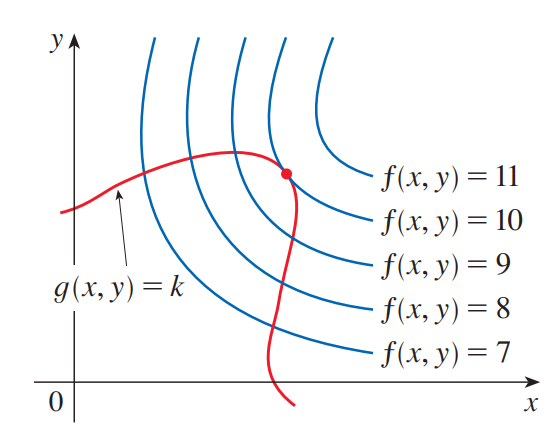
\includegraphics[width=0.5\linewidth]{images/geometric-meaning-lagrange-multiplier.png}
    \caption{Geometric Meaning of Lagrange Multipliers}
    \label{fig:geometric-meaning-lagrange-multiplier}
\end{figure}
\begin{notebox}
    \begin{remark}
        Note that both the {\color{blue} \textbf{blue}} lines and {\color{red} \textbf{red}} lines in the figure \ref{fig:geometric-meaning-lagrange-multiplier} are the {\color{red} \textbf{level curves}} of the original functions $f(x,y)$ and $g(x,y)$. And the reason we do {\color{red} \textbf{level curves}} is that we want to find the value of $x$ and $y$ that enable us to achieve the maximum/minimum value. Under this circumstance, {\color{red} \textbf{level curves}} of the graphs of these two functions are the most useful.
    \end{remark}
\end{notebox}
\subsubsection{Method of Lagrange Multipliers}
\begin{thmbox}{Method of Lagrange Multipliers}{method-of-lagrange-multipliers}
    To find the maximum and minimum values of $f(x,y,z)$ subject to the constraint $g(x,y,z)=k$ [assuming that these extreme values exist and $\nabla g \neq 0$ on the surface $g(x,y,z)=k$]:
    \begin{enumerate}
        \item Find all values of $x,y,z$ and $\lambda$ such that
        \begin{displaymath}
            \nabla f(x,y,z) = \lambda \nabla g(x,y,z)
        \end{displaymath}
        and
        \begin{displaymath}
            g(x,y,z)=k
        \end{displaymath}
        \item Evaluate $f$ at all the points $(x,y,z)$ that result from step 1. The largest of these values is the maximum value of $f$; the smallest is the minimum of $f$.
    \end{enumerate}
\end{thmbox}
\subsection{Two Constraints}
We only need to modify our \nameref{thm:method-of-lagrange-multipliers} into
\begin{displaymath}
    \nabla f(x,y,z)=\lambda \nabla g(x,y,z) + \mu \nabla h(x,y,z)
\end{displaymath}
and let the two constraints satisfy simultaneously.
\end{document}